%!TEX root = article.tex
We report the proofs of the different propositions (\autoref{sec:proofs}), an instantiation of online Sinkhorn for discrete measures (\autoref{sec:sinkhorn_discrete}), and a supplementary experiment (\autoref{sec:supp_exp}).

\section{Proofs}\label{sec:proofs}

We first introduce two useful known lemmas, and prove the propositions in their order of appearance.

\subsection{Useful lemmas}

First, under \autoref{ass:lip}, we note that the soft $C$-transforms are
 uniformly contracting on the distribution space $\Pp(\Xx)$. This is clarified
 in the following lemma, extracted from \citet{vialard2019elementary},
 Proposition 19. We refer the reader to the original references for proofs.

\begin{lemma}\label{lemma:contractance}
    Unser \autoref{ass:lip}, let $\kappa = 1 - \exp(-L
    \textnormal{diam}(\Xx))$. For all $\hat \alpha \in \Pp(\Xx)$ and $\hat \beta \in
    \Pp(\Xx)$, for all $f, f', g, g' \in \Cc(\Xx)$,
    \begin{equation}
        {\Vert \Ctrans{f'}{\hat \alpha} - 
        \Ctrans{f'}{\hat \alpha} \Vert}_{\var} \leq \kappa {\Vert f - f' \Vert}_{\var},
        \quad
        {\Vert \Ctrans{g}{\hat \beta} - 
        \Ctrans{g'}{\hat \beta} \Vert}_{\var} \leq \kappa {\Vert g - g' \Vert}_{\var}.
    \end{equation}
\end{lemma}

We will also need a uniform law of large numbers for functions. The following lemma is a consequence of Example 19.7 and
Lemma 19.36 of \citet{van_der_vaart_asymptotic_2000}, and is copied in Lemma B.6 in \citet{mairal_stochastic_2013}.

\begin{lemma}\label{lemma:lln}
    Under \autoref{ass:lip}, let $(f_t)_t$ be an i.i.d sequence in $\Cc(\Xx)$,
    such that $\EE[f_0] = f \in \Cc(\Xx)$. Then there exists $A > 0$ such that, for all $n > 0$,
    \begin{equation}
        \EE \sup_{x \in \Xx} | \frac{1}{n} \sum_{i=1}^n f_i(x) - f(x) |
        \leq \frac{A}{\sqrt{n}}.
    \end{equation}
\end{lemma}
Finally, we need a result on running averages using the sequence ${(\eta_t)}_t$. The following result stems from a simple Abel transform of the law of large number, and is established by \citet{mairal_stochastic_2013}, Lemma B.7.

\begin{lemma}\label{lemma:running}
    Let $(\eta_t)_t$ be a sequence of weights meeting \autoref{ass:weights}. Let
    $(X_t)_t$ be an i.i.d sequence of real-valued random variables with existing
    first moment $\EE[X_0]$. We consider the sequence ${(\bar X_t)}_t$ defined
    by $\bar X_0 \triangleq X_0$ and 
    \begin{equation}
        \bar X_t \triangleq (1 - \eta_t) \bar X_{t-1} + \eta_t X_t.
    \end{equation}
    Then $\bar X_t \to_{t \to \infty} \EE[X_0]$.
\end{lemma}

\subsection{Proof of \autoref{prop:markov}}\label{sec:proof_markov}

\begin{proof}
    We use Theorem 1 from \citet{diaconis_iterated}. For this, we simply note
    that the space $\Cc(\Xx) \times \Cc(\Xx)$ in which the chain ${x_t
    \triangleq (f_t, g_t)}_t$, endowed with the metric $\rho((f_1, g_1), (f_2,
    g_2)) = \Vert f_1 - f_2 \Vert_{\var} + \Vert g_1 - g_2 \Vert_{\var}$, is
    complete and separable (the countable set of polynomial functions are dense in this space, for example).
    We consider the operator $A_{\theta} \triangleq \Ctrans{\Ctrans{\cdot}{\hat
    \alpha}}{\hat \beta}$. $\theta \triangleq (\hat \alpha, \hat \beta)$ denotes
    the random variable that is sampled at each iteration. We have the following
    recursion:
    \begin{equation}
        x_{t+2} = A_{\theta_t}(x_t).
    \end{equation}
    
    From \autoref{lemma:contractance}, for all $\hat \alpha \in \Pp(\Xx)$, $\hat \beta \in \Pp(\Xx)$, $A_{\theta}$
    with $\theta = (\hat \alpha, \hat \beta)$ is contracting, with module
    $\kappa_\theta < \kappa < 1$. Therefore
    \begin{equation}
        \int_{\theta} \kappa_\theta \d \mu(\theta) < 1, \qquad \int_{\theta}
         \log \kappa_\theta \d \mu(\theta) < 0.
    \end{equation}
    Finally, we note, for all $f \in \Cc(\Xx)$
    \begin{equation}
        \Vert \Ctrans{\Ctrans{f}{\hat \alpha}}{\beta} \Vert_{\infty} 
        \leq \Vert f \Vert_\infty + 2 \max_{x,y \in \Xx} C(x, y),
    \end{equation}
    therefore $\rho(A_\theta(x_0), x_0) \leq 2 \Vert x_0 \Vert_\infty + 2
    \max_{x,y \in \Xx} C(x, y)$ for all $\theta \ (\hat \alpha, \hat \beta)$.
    The regularity condition of the theorem are therefore met. Each of the
    induced Markov chains ${(f_{2t}, g_{2t})}_t$ and ${(f_{2t + 1}, g_{2t +
    1})}_t$ has a unique stationary distribution. These stationary distributions
    are the same: the stationary distribution is independent of the
    initialisation and both sequences differs only by their initialisation.
    Therefore ${(f_{t}, g_{t})}_t$ have a unique stationary distribution
    $(F_\infty, G_\infty)$.
\end{proof}

\subsection{Proof of \autoref{prop:convergence_approx}}\label{sec:proof_convergence_approx}


For presentation purpose, we first show that the ``slowed-down'' online Sinkhorn algorithm converges in the absence of noise. We then turn to prove \autoref{prop:convergence_approx}.

\subsubsection{Noise-free online Sinkhorn}

\begin{proposition}\label{prop:deterministic}
    We suppose that $\hat \alpha_t = \alpha$, $\hat \beta_t = \beta$ for all
    $t$. Then the updates \eqref{eq:updates} yields a (deterministic) sequence $(f_t, g_t)_t$ such
    that 
    \begin{equation}
        \Vert \hat f_t - f^\star \Vert_{\text{var}} 
        + \Vert \hat g_t - g^\star \Vert_{\text{var}} \to 0,\qquad
        \frac{1}{2} \dotp{\alpha}{f_t + \Ctrans{\hat g_t}{\alpha}} + \dotp{\beta}{\hat g_t + \Ctrans{f_t}{\beta}} 
         \to \Ww(\alpha, \beta).
    \end{equation}
\end{proposition}
Note that, as we perform \textit{simultaneous} updates, we only obtain
the convergence of $f_t \to f^\star + A$, and $g_t \to g^\star$, where $f^\star$
and $g^\star$ are solutions of \eqref{eq:wass} and $A$ is a constant depending
on initialization.
%%%

The \enquote{slowed-down} Sinkhorn iterations converge toward an optimal
potential couple, up to a constant factor: this stems from the fact that we
apply contractions in the space $(\Cc(\Xx), {\Vert\cdot\Vert}_{\var})$ with a
contraction factor that decreases sufficiently slowly.

\begin{proof}
    We write ${(f_t, g_t)}_t$ the sequence of iterates. Given a pair of optimal potentials 
    $(f^\star, g^\star)$, we write $u_t \triangleq f_t - f^\star$, $v_t \triangleq g_t - g^\star$,
    $u_t^T \triangleq \Ctrans{f_t}{\alpha} - g^\star$ and $v_t^T \triangleq \Ctrans{g_t}{\alpha} - f^\star$.
    For all $t > 0$, we observe that 
    \begin{align}
        \max u_{t+1} &= - \log \min \exp(-u_{t+1}) \\
        &= - \log \big( \min \big( (1 - \eta_t) \exp(-u_{t}) + \eta_t 
        \exp(-v_t^T) \big) \big)\\
        &\leq - \log \big( (1 - \eta_t) \min \exp(-u_{t}) + \eta_t 
        \min \exp(-v_t^T) \big)\\
        &\leq - (1 - \eta_t) \log \min \exp(-u_{t}) -  \eta_t \log \min
         \exp(-v_t^T) \\
         &= (1 - \eta_t) \max u_t  + \eta_t \max v_t^T,
    \end{align}
    where we have used the algorithm recursion on the second line, $\min f + g \geq \min f + \min g$
     on the third line and Jensen inequality on the fourth line. Similarly
    \begin{equation}
        \min u_{t+1} \geq (1 - \eta_t) \min u_t  + \eta_t \min v_t^T,
    \end{equation}
    and mirror inequalities hold for $v_t$. Summing the four inequalities, we obtain
    \begin{align}\label{eq:et}
        e_{t+1} &\triangleq \Vert u_{t+1} \Vert_{\var} + \Vert v_{t+1} \Vert_{\var} \\ 
        &= \max u_{t+1} - \min u_{t+1} + \max v_{t+1} - \min v_{t+1} \\
        &\leq
        (1 - \eta_t) ( \Vert u_t \Vert_{\var} + \Vert v_t \Vert_{\var})
        + \eta_t ( \Vert u_t^T \Vert_{\var} + \Vert v_t^T \Vert_{\var}), \\
        &\leq
        (1 - \eta_t) ( \Vert u_t \Vert_{\var} + \Vert v_t \Vert_{\var})
        + \eta_t \kappa ( \Vert u_t \Vert_{\var} + \Vert v_t \Vert_{\var}),
    \end{align}
    where we use the contractance of the soft-$C$-transform, that guarantees that
    there exists $\kappa < 1$ such that $\Vert v_t^T\Vert_{\var} \leq \kappa \Vert
    v_t\Vert_{\var}$ and $\Vert u_t^T\Vert_{\var} \leq \kappa \Vert
    u_t\Vert_{\var}$ \citep{peyre2019computational}.

    Unrolling the recursion above, we obtain
    \begin{equation}
        \log e_t = \sum_{s=1}^t \log(1 - \eta_t (1 - \kappa)) + \log(e_0) \to - \infty,
    \end{equation}
    provided that $\sum \eta_t = \infty$. The proposition follows.
\end{proof}


\begin{proof}[Proof of \autoref{prop:convergence_approx}]
For discrete realizations $\hat \alpha$ and $\hat \beta$, we define the perturbation terms
\begin{equation}
    \epsilon_{\hat \beta}(\cdot) \triangleq
    f^\star - \Ctrans{g^\star}{\hat \beta} ,\qquad
    \iota_{\hat \alpha}(\cdot) \triangleq 
    g^\star - \Ctrans{f^\star}{\hat \alpha},
\end{equation}
so that the updates can be rewritten as
\begin{align}
    \exp(-f_{t+1} + f^\star) &= (1 - \eta_t)
    \exp(-f_{t} + f^\star)
    + \eta_t \exp(-\Ctrans{g_t}{\hat \beta_t} 
    +\Ctrans{g^\star}{\hat \beta_t} + \epsilon_{\hat \beta_t}) \\
    \exp(-g_{t+1} + g^\star) &= (1 - \eta_t)
    \exp(-g_{t} + g^\star)
    + \eta_t \exp(-\Ctrans{f_t}{\hat \alpha_t} 
    +\Ctrans{f^\star}{\hat \alpha_t} + \iota_{\hat \alpha_t}).
\end{align}
We denote $u_t \triangleq -f_{t} + f^\star$, $v_t \triangleq -g_{t} + g^\star$, $u_t^T \triangleq
\Ctrans{f_t}{\hat \beta_t} - \Ctrans{f^\star}{\hat \beta_t}$, $v_t^T \triangleq
\Ctrans{g_t}{\hat \beta_t} - \Ctrans{g^\star}{\hat \beta_t}$. Reusing the same
derivations as in the proof of \autoref{prop:deterministic}, we obtain
    \label{eq:pre_ineq_var}
    \begin{align}
    \Vert u_{t+1} \Vert_{\var} &\leq
    (1 - \eta_t) \Vert u_t \Vert_{\var}
    \\
    &\phantom{=}+ \eta_t \log \big( \max_{x, y \in \Xx}
    \exp(\epsilon_{\hat \beta_t}(x) 
    - \epsilon_{\hat \beta_t}(y)) \exp(v_t^T(x) - v_t^T(y)) \big) \\ 
    &\leq
    (1 - \eta_t) \Vert u_t \Vert_{\var}
    + \eta_t \Vert v_t^T \Vert_{\var}
    + \eta_t \Vert \epsilon_{\hat \beta_t} \Vert_{\var},
\end{align}
where we have used $\max_x f(x) g(x) \leq \max_x f(x) \max_x f(x)$ on the second line. Therefore,
using the contractance of the soft $C$-transform,
\begin{equation}
    \label{eq:ineq_var}
    e_{t+1} \leq 
    (1 - \tilde \eta_t) e_t
    +  \frac{\tilde \eta_t}{1 -\kappa}
    ({\Vert \epsilon_{\hat \beta_t} \Vert}_{\var} + 
    {\Vert \iota_{\hat \alpha_t} \Vert}_{\var}),
\end{equation}
where we set $e_t \triangleq \Vert u_t \Vert_{\var} + \Vert v_t \Vert_{\var}$,
$\tilde \eta_t = \eta_t (1-\kappa)$ and $\kappa$ is set to be the biggest
contraction factor over all empirical realizations $\hat \alpha_t$, $\hat
\beta_t$ of the distributions $\alpha$ and $\beta$. It is upper bounded by $1 -
e^{- L\text{diam}(\Xx)}$, thanks to \autoref{ass:lip} and
\autoref{lemma:contractance}.

The realizations $\hat \beta_t$ and $\hat \alpha_t$
are sampled according to the same distribution $\hat \alpha$ and $\hat \beta$. We
define the sequence $r_t$ to be the running average of the variational norm of the
(functional) error term:
\begin{equation}
    r_{t+1} \triangleq (1 - \tilde \eta_t) r_t + \frac{\tilde \eta_t}{1 - \kappa}
    ({\Vert \epsilon_{\hat \beta_t} \Vert}_{\var} + 
    {\Vert \iota_{\hat \alpha_t} \Vert}_{\var}).
\end{equation}
We thus have, for all $t > 0$, $e_t \leq r_t$. Using \autoref{lemma:running}, the sequence $(r_t)_t$
converges towards the scalar expected value
\begin{equation}\label{eq:r_infty}
    r_\infty \triangleq \frac{1}{1 - \kappa} \EE_{\hat \alpha, \hat \beta}[{\Vert \epsilon_{\hat \beta} \Vert}_{\var}
    + {\Vert \iota_{\hat \alpha} \Vert}_{\var}] > 0.
\end{equation}
We now relate $r_\infty$ to the number of samples $n$ using
a uniform law of large number result on parametric functions.
We write $\hat \beta = \hat \beta_n$ to make explicit the dependency of the
quantities on the batch size $n$.

Using \autoref{lemma:lln}, we bound the quantity
\begin{align}
    E_n &\triangleq \EE_{\hat \beta_n} {\Vert \epsilon_{\hat \beta_n} \Vert}_{\var}
     = \EE_{\hat \beta_n} {\Vert \exp(-\Ctrans{g^\star_0}{\beta})
    - \exp(-\Ctrans{g^\star_0}{\hat \beta_n}) \Vert}_{\infty} \\
    &= \EE_{Y_1, \dots Y_n \sim \beta} 
    \sup_{x \in \Xx}
     \Big| \frac{1}{n} \sum_{i=1}^n \exp(g^\star(Y_i)) - C(x, Y_i)) \\
      &\phantom{=}\qquad\qquad\qquad\quad- \EE_{Y \sim \beta}[\exp(g^\star_0(Y)) - C(x, Y)] \Big| \\
      &= \EE \sup_{x \in \Xx} | \frac{1}{n} \sum_{i=1}^n \phi_i(x) - \phi(x) | ,
\end{align}
where we have defined $\phi_i: x \to \exp(g^\star(Y_i) - C(x, Y_i))$ and set
$\phi$ to be the expected value of each $\phi_i$. The compactness of $\Xx$
ensures that the functions  are square integrable and uniformly bounded.
\autoref{lemma:lln} ensures that there exists $S(g^\star)$ such that
\begin{equation}
    E_n \leq \frac{S(g^\star)}{\sqrt{n}}.
\end{equation}
We now bound $\EE_{\hat \beta_n} {|| \epsilon_{\hat \beta_n} ||}_\var$ using the
 quantity $E_n$. First, we observe that $\Vert_{\var} = g^\star_{\min} < g^\star
 < 0$, and there exists $C_{\max} > 0$ such that $0 \leq C(x, y) \leq C_{\max}$
 for all $x, y \in \Xx$, thanks to the \autoref{ass:lip}.
 \begin{align}
    \delta \triangleq \exp(-\Vert g^\star \Vert_{\var}
     - C_{\max}) &\leq \exp(-T_\beta(g^\star)) \leq 1 \\
    \exp(-\Vert g^\star \Vert_{\var}
     - C_{\max}) &\leq \exp(-T_{\hat \beta_n} 
    (g^\star)) \leq 1,
\end{align}
where we have used $g^\star = \Vert g^\star \Vert_{\var}$.
For all $x \in \Xx$, 
\begin{equation}\label{eq:expression}
    | \epsilon_{\hat \beta_n} | = 
    | \log \frac{\exp(-T_{\hat \beta_n}(g^\star))}{\exp(-T_\beta(g^\star))} | =
    \Big| \log\big(1 + 
    \frac{\exp(-\Ctrans{g^\star}{\hat \beta_n})
    -\exp(-\Ctrans{g^\star}{\beta})
    }
    {\exp(-\Ctrans{g^\star}{\beta})}\big) \Big|.
\end{equation}
We first obtain an upper-bound independent of $n$ with the first equality in
 \eqref{eq:expression}:
\begin{equation}\label{eq:const_ineq}
    {|| \varepsilon_{\hat \beta_n} ||}_{\var} \leq {|| \varepsilon_{\hat \beta_n} ||}_{\infty} \leq 
    {\Vert g^\star \Vert}_{\var} + C_{\max}.
\end{equation}
 We now use the second expression in \eqref{eq:expression}: for $n$ large enough, $E_n < \delta$
\begin{equation}\label{eq:log_ineq}
    {|| \varepsilon_{\hat \beta_n} ||}_{\var} \leq \max ( \log(1 + \frac{E_n}{\delta}),
     - \log(1 - \frac{E_n}{\delta}) ) = 
    - \log(1 - \tilde E_n),
\end{equation}
where we have set $\tilde E_n \triangleq \frac{E_n}{\delta}$. On the event
$\Omega_n = \{\tilde E_n \leq \frac{1}{2}\}$, a simple calculation gives $- \log(1
- \tilde E_n) \leq (2 \log 2) \tilde E_n \leq 2 \tilde E_n$. Thanks to Markov inequality,
$\PP[\tilde E_n > \frac{1}{2}] \leq 2 \EE[\tilde E_n]$. We then split the
expectation over the event $\Omega_n$, and use inequalities \eqref{eq:log_ineq}
and \eqref{eq:const_ineq} on each conditional expectation:
\begin{align}\label{eq:vdv}
    \EE {|| \varepsilon_{\hat \beta_n} ||}_{\var}  &= \PP\left[\tilde E_n \leq \frac{1}{2}\right] 
    \EE \left[ {|| \varepsilon_{\hat \beta_n} ||}_{\var}
    \Big| \tilde E_n \leq \frac{1}{2}\right] 
    \\
    &\phantom{=}
    + \PP\left[\tilde E_n > \frac{1}{2}\right]      \EE \left[ {|| \varepsilon_{\hat \beta_n} ||}_{\var}
    \Big| \tilde E_n > \frac{1}{2}\right] \\
    &\leq \frac{2 \phi({\Vert g^\star \Vert}_{\var} + C_{\max}) 
    S(g^\star)}{\sqrt{n}}\\
    &\leq \frac{4 \exp({\Vert g^\star \Vert}_{\var} + C_{\max}) 
    S(g^\star)}{\sqrt{n}} \triangleq \frac{A(g^\star)}{\sqrt{n}}
\end{align}
The constants $S$ depends on the complexity of estimating
the functional $x \to \int_y \exp(g^\star(y) - C(x,y)) \d \beta(y)$ with samples from $\beta$.
A parallel
result holds for $\EE_{\hat \alpha_n} {\Vert \iota_{\hat \alpha_n}
\Vert}_{\var}$. There exists $A(f^\star), A(g^\star) > 0$ such that $r_\infty \leq
\frac{A(f^\star) + A(g^\star)}{\sqrt{n}}$. As for all $t >0$, $e_t \leq r_t \to_{t \to \infty}
r_\infty$, the proposition follows,  writing $A = A(f^\star) + A(g^\star)$.

The constant $A$ is larger than $\exp(C_{\max})$ when $C_{\max} \to
\infty$; Hence it behaves at least like $\exp(\frac{1}{\varepsilon})$ when~$\varepsilon
\to 0$.

Note that we have used twice a corollary of the law of large numbers: once when
averaging over $t$ with $t \to \infty$ (Eq. \eqref{eq:r_infty}), and once when
averaging over $n$ with $n$ finite (Eq. \eqref{eq:vdv}).
\end{proof}

\subsection{Proof of \autoref{prop:convergence_true}}\label{sec:proof_prop_convergence}

In the proof of \autoref{prop:convergence_approx} and in particular Eq. \eqref{eq:ineq_var}, the term that prevents the convergence of $e_t$ is
\begin{equation}
    \eta_t ({\Vert \epsilon_{\hat \beta_t} \Vert}_{\var} + 
    {\Vert \iota_{\hat \alpha_t} \Vert}_{\var}),
\end{equation}
which is not summable in general. We can control this term by increasing the
 size of $\hat \alpha_t$ and $\hat \beta_t$ with time, at a sufficient rate: this is what \autoref{ass:double_weights} ensures.

\begin{proof}
From Eq. \eqref{eq:ineq_var}, for all $t > 0$, we have
\begin{equation}\label{eq:Et_rec}
    0 \leq e_{t+1} \leq 
    (1 - \tilde \eta_t) e_t
    + \eta_t
    ({\Vert \epsilon_{\hat \beta_t} \Vert}_{\var} + 
    {\Vert \iota_{\hat \alpha_t} \Vert}_{\var}).
\end{equation}
Taking the expectation and using the uniform law of 
large number \eqref{eq:vdv},
\begin{align}\label{eq:recursion}
    \EE e_{t+1} &\leq (1 - (1 - \kappa) \eta_t) \EE e_t + 
    \eta_t \frac{A}{\sqrt{n(t)}} \\
    &= (1 - (1 - \kappa) \eta_t) \EE e_t + 
    A \eta_t w_t,
\end{align}
where we have used the definition of $n(t)$ from \autoref{ass:double_weights} in the last line.

The proof follows from a simple asymptotic analysis of the sequence ${(\EE e_t)}_t$, following recursion \eqref{eq:recursion}.
For all $t > 0$, 
\begin{equation}\label{eq:Et_rec2}
    \EE e_{t+1} - \EE e_t = - (1 - \kappa) \eta_t \EE e_t + A \eta_t w_t
     \leq A \eta_t w_t
\end{equation}
Therefore, from \autoref{ass:double_weights}, ${(\EE e_{t+1} - \EE e_t)}_t$ is
summable and $\EE e_t \to_{t \to \infty} \ell \geq 0$. Let's assume $\ell > 0$.
Summing \eqref{eq:Et_rec2} over $t$, we obtain
\begin{equation}
    \EE e_t \leq \EE e_1 - (1 - \kappa) \sum_{s=1}^{t-1} \eta_s \EE_s 
    + A \sum_{s=1}^{t-1} \eta_s w_s \to_{t \to \infty} - \infty,
\end{equation}
which leads to a contradiction. Therefore $\EE e_t \to_{t \to \infty} 0$. As
$e_t \geq 0$ for all $t > 0$, this implies that $e_t \to_{t \to \infty} 0$
almost surely.
\end{proof}


\subsection{Proof of \autoref{prop:rate}}\label{app:proof_rate}

\begin{proof}
The proof of \autoref{prop:convergence_true} allows us to derive non-asymptotic rates for potential estimations using the online Sinkhorn algorithm. Let us set $\eta_t = \frac{\lambda}{t^a}$, $n(t) = \lceil B t^{2b} \rceil$ in \eqref{eq:Et_rec}, so that \autoref{ass:double_weights} is met.
$\lceil \cdot \rceil$ denotes the ceiling function.
We are left to study the recursion \eqref{eq:recursion}:
\begin{equation}
    \delta_{t+1} \triangleq \EE e_{t+1} \leq (1 - \frac{\lambda(1 - \kappa)}{t^a}) \delta_t + 
    \frac{A \lambda}{\sqrt{B}{t^{a + b}}}
\end{equation}

Following the derivations of \citet[Theorem 2]{moulines_non-asymptotic_2011}, we have the following
bias-variance decomposed upper-bound,
provided that $0 \leq a < 1$ and $a+ b > 1$. For all $t > 0$,
% \begin{equation}
%     \delta_t \leq (\delta_0 + \frac{A S}{\sqrt{B}} \phi_{1 - (a + b)}(t))
%     \exp(- \frac{S(1 - \kappa)}{2} n^{1 - a})
%     + \frac{2 A S}{\sqrt{B}(1 - \kappa) n^a}, 
% \end{equation}
% where $\phi_c(t) = \frac{t^c - 1}{c}$ for all $c \neq 0$, $\phi_0(t) = \log t$.
% Note that $\phi_{1 - (a + b)} \leq \frac{1}{a + b - 1}$, so that
\begin{equation}\label{eq:rates}
    \delta_t \leq (\delta_0 + \frac{A S}{(a + b - 1)\sqrt{B}})
    \exp(- \frac{S(1 - \kappa)}{2} t^{1 - a})
    + \frac{2 A S}{\sqrt{B}(1 - \kappa) t^a}.
\end{equation}
Let us now relate the iteration number $t$ to the number of seen sample $N$. By definition
\begin{equation}
    n_t = \sum_{s=1}^t n(s) \leq B \sum_{s=1}^t s^{2b} + t \leq
     t + \frac{(t+1)^{2b + 1} - 1}{2b + 1}
     \leq (2t)^{2b+1}.
\end{equation}
Therefore, when we have seen $N$ samples, the iteration number is superior to $t(N)$, and the expected error $\delta_N$ is of the order of $\delta_{t(N)}$, with
\begin{equation}\label{eq:tn}
    t(N) =  {(N/2)}^{\frac{1}{2b + 1}}.
\end{equation}
We write $\delta_N = \delta_{t(N)}$. Replacing \eqref{eq:tn} in \eqref{eq:rates} yields
\begin{equation}\label{eq:non-asymptotic}
    \delta_n \leq 
    (\delta_0 + \frac{A \lambda}{(a + b - 1)\sqrt{B}})
    \exp\left(- \frac{\lambda(1 - \kappa)}{2} {(n /2)}^{\frac{1 - a}{2b+1}}\right)
    + \frac{2 A \lambda}{\sqrt{B}(1 - \kappa) {(n/2)}^{\frac{a}{2b+1}}}.
\end{equation}
We note that $b$ and $a$ should be as close to $0$ as possible to reduce the bias term, while $a$
should be as close to $1$ and $b$ as close to $0$ as possible to reduce the variance
term. Of course, $b$ should remain larger than $1 - a$ to ensure convergence.

To obtain the best asymptotical rates (the error is always dominated by the variance term), we set $a = 1 - \iota$, $ b = 2 \iota$, with $\iota \succsim 0$. This yields
\begin{align}
    \delta_n &\leq 
    (\delta_0 + \frac{A \lambda}{\iota \sqrt{B}})
    \exp\left(- \frac{\lambda(1 - \kappa)}{2} {(n/2)}^{\frac{\iota}{1 + 4\iota}}\right)
    + \frac{2 A \lambda}{\sqrt{B}(1 - \kappa) {(n/2)}^{\frac{1 - \iota}{1 + 4\iota}}} \\
    &= \Oo(n^{-\frac{1 - \iota}{1 + 4 \iota}}).
\end{align}

This rate is as close to the rate $\Oo(\frac{1}{n})$ as desired. We may then
perform a last soft $C$-transform (using the $n_t$ seen samples) over the
estimated $f_{t(n)}, g_{t(n)}$ to obtain a estimated solution of the dual
optimisation problem \eqref{eq:dual}. The Sinkhorn potentials can therefore be
estimated with \textit{fast rates}. Note that the upper bound explodes when $\varepsilon
\to 0$, as $C_{\max} \to \infty$, hence $A \to \infty$, and $(1 - \kappa) \to 0$.
\end{proof}

\paragraph{Estimating the Sinkhorn distance.} The Sinkhorn distance requires to estimate the integral
\begin{equation}
    \Ww(\alpha, \beta) = \int_x f^\star(x) \d \alpha(x) + \int_y g^\star(y) \d \beta(y).
\end{equation}
At iteration $t(n)$, with empirical realization $\bar \alpha_t$ and $\bar
\beta_t$, containing $n$ samples, we use the estimator
\begin{equation}
    \hat \Ww(\alpha, \beta) = \frac{1}{n} \sum_{i=1}^n f_{t(n)}(x_i) + \frac{1}{n} \sum_{i=1}^n g_{t(n)}(y_i),
\end{equation}
We can bound the estimation error $|\hat \Ww(\alpha, \beta) - \Ww(\alpha, \beta)
| = \Oo(\frac{1}{\sqrt{n}})$, dominated by the integral evaluation noise. We
thus recover a new estimator of the Sinkhorn distance with the same sample
complexity as the batch Sinkhorn estimator \citep{2019-Genevay-aistats}. Our
estimator enjoys an original rate for estimating the potentials in $\Vert \cdot
\Vert_{\var}$.

\pagebreak
\section{Online Sinkhorn variants}

\subsection{Fully-corrective scheme}\label{app:fully_corrective}

We report the fully-corrective online Sinkhorn algorithm in \autoref{alg:full_corrective}. This algorithm also enjoys almost sure convergence, provided that the following assumption is met.

\begin{algorithm}[t]
    \begin{algorithmic}
    \State \textbf{Input:} Distribution $\alpha$ and $\beta$, learning weights ${(\eta_t)}_t$ and batch-sizes ${(n(t))}_t$. 
    \textbf{Set} $p_{i,1} = q_{i,1} = 0$ for $i \in (0, n_1]$
    \For{$t= 0, \dots, {T-1}$}
        \State Sample $(x_i)_{(n_t, n_{t+1}]} \sim \alpha$, $(y_j)_{(n_t, n_{t+1}]} \sim \beta$.
            \State Evaluate $(\hat f_t(x_i))_{i=(0, n_{t+1}]}$,
             $(\hat g_t(y_i))_{i=(0, n_{t+1}]}$ using $(q_{i,t}, p_{i,t}, x_i, y_i)_{i=(0,n_{t}]}$ in \eqref{eq:param}.
             \State $q_{(0, n_{t+1}],t+1} {\gets} \log \frac{1}{n}
             + (\hat g_t(y_i))_{(0, n_{t+1}]}$,
             \qquad $p_{(n_t, n_{t+1}],t+1} {\gets} \log \frac{1}{n} 
             + (\hat f_t(x_i))_{(n_t, n_{t+1}]}$.
    \EndFor
    \State \textbf{Returns:} $\hat f_T : (q_{i,T}, y_i)_{(0, n_T]}$ and
    $\hat g_T : (p_{i,T}, x_i)_{(0, n_T]}$
    \end{algorithmic}
    \vspace{-.4em}
    \caption{Fully-corrective online Sinkhorn}\label{alg:full_corrective}
\end{algorithm}

\begin{algorithm}[t]
    \begin{algorithmic}
    \Input Distribution $\alpha \in \triangle^N$ and 
    $\beta \in \triangle^N$, $x \in \RR^{n \times d}$, 
    $y \in \RR^{n \times d}$, learning weights ${(\eta_t)}_t$
    \State \textbf{Set} $p = q = - \infty \in \RR^n$.
    \For{$t= 1, \dots, {T}$}
        \State $q \gets q + \log(1 - \eta_t)$, $p \gets p + \log(1 - \eta_t)$.
        \State Sample $J_t \subset [1, N]$, $I_t \subset [1, N]$ of size $n(t)$.
        \For{$i \in J_t$}
            \State $q_i \gets \log \Big( \exp(q_i)
            + \exp\big(\log(\eta_t) - \log \frac{1}{N} 
            \sum_{j=1}^{N} \exp(p_j - C(x_j, y_i)\big) \Big) $.
        \EndFor
        \For{$i \in I_t$}
        \State $p_i \gets \log \Big( \exp(q_i)
        + \exp \big( \log(\eta_t) - \log \frac{1}{M} 
        \sum_{j=1}^{M} \exp(q_j - C(x_i, y_j)\big) \Big)$.
        \EndFor
    \EndFor
    \State Returns $f_T : (q, y)$ and
    $g_T : (p, x)$
    \end{algorithmic}
    \caption{Online Sinkhorn potentials in the discrete setting}\label{alg:discrete_online}
\end{algorithm}

\begin{assumption}\label{ass:total_growing}
    For all $t > 0$, the \textit{total} batch-size $n_t = \frac{B}{w_t^2}$ is an
        integer. The step-size $\eta_t$ and the batch-size $n_t$ grows so that
        $\sum w_t \eta_t < \infty$ and $\sum \eta_t = \infty$.
\end{assumption}

With full correction, the total number of observed samples $n_t$ needs to grow
at the same rate as the single-iteration batch-size $n(t)$ in
\autoref{ass:double_weights}. For $\eta_t = \frac{1}{t^a}$, $a \in (1/2, 1]$, it
is sufficient to use a constant batch-size $n(t) = B$ to meet \autoref{ass:total_growing}. We then have the following property

\begin{proposition}
    Under \autoref{ass:lip} and
    \ref{ass:total_growing}, the fully-corrective online Sinkhorn algorithm converges almost surely:
    \begin{equation}
        \Vert \hat f_t - f^\star \Vert_{\var} + \Vert \hat g_t - g^\star \Vert_{\var} \to 0.
    \end{equation}
\end{proposition}



\subsection{Online Sinkhorn for discrete distributions}\label{sec:sinkhorn_discrete}

The online Sinkhorn algorithm takes a simpler form with discrete
distributions. We derive it in \autoref{alg:discrete_online}. We set $\alpha$
and $\beta$ to have size $N$ and $M$, respectively. We evaluate
the potentials as
\begin{align}
    g_t(y) &= - \log \sum_{j=1}^N \exp(p_j - C(x_j, y)) \\
    f_t(x) &= - \log \sum_{j=1}^M \exp(q_j - C(x, y_j)), \\
\end{align}

\vspace{-2em}
where $(p_j)_{J \in [1, N]}$ and $(q_j)_{J \in [1, M]}$ are fixed-size vectors.
Note that the computations written in \autoref{alg:discrete_online} are
in log-space,as they should be implemented to prevent numerical overflows. The sets $|I|$ and $|J|$ can
have varying sizes along the algorithm, which allows for example to speed-up the
initial Sinkhorn iteration (\autoref{sec:accelerating}). In this case, the
cost matrix $\hat C = C(x_i,y_j))_{i,j}$ should be progressively recorded along the algorithm iterations.

\pagebreak
\section{Supplementary numerical experiments}

We report the supplementary figures mentionned in the main text, as well as experimental details.

\subsection{All convergence curves for online Sinkhorn and variants}\label{app:online_exp}

\begin{figure}[t]
    \centering
    $\varepsilon = 0.1$

    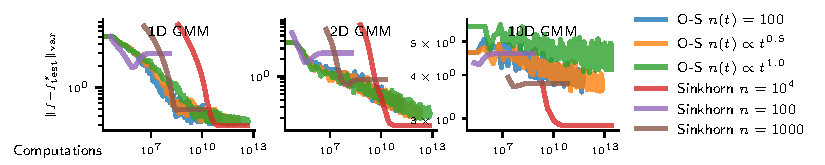
\includegraphics{online_0.1_False_test}
    
    $\varepsilon = 0.01$
    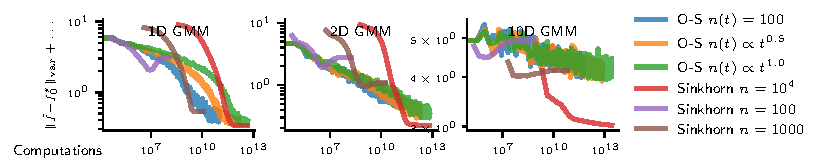
\includegraphics{online_0.01_False_test}

    $\varepsilon = 0.001$

    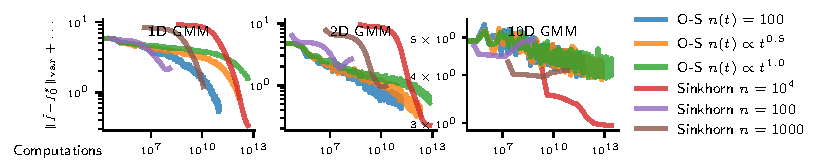
\includegraphics{online_0.001_False_test}

    $\varepsilon = 0.0001$

    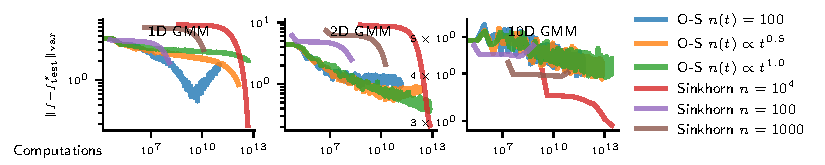
\includegraphics{online_0.0001_False_test}
    \caption{Performance of online Sinkhorn for various $\varepsilon$.}
    \label{fig:convergence_all}
\end{figure}

\begin{figure}[t]
    \centering
    $\varepsilon = 0.1$

    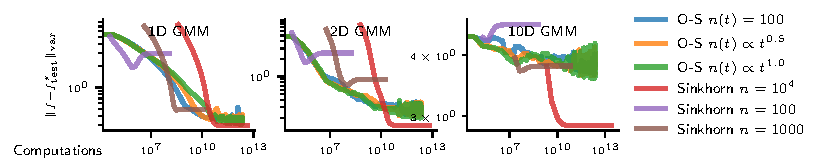
\includegraphics{online_0.1_True_test}
    
    $\varepsilon = 0.01$
    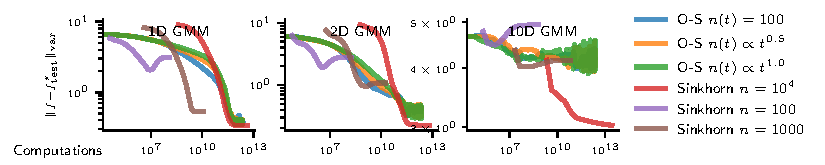
\includegraphics{online_0.01_True_test}

    $\varepsilon = 0.001$

    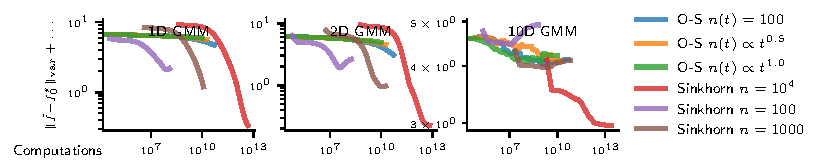
\includegraphics{online_0.001_True_test}

    $\varepsilon = 0.0001$

    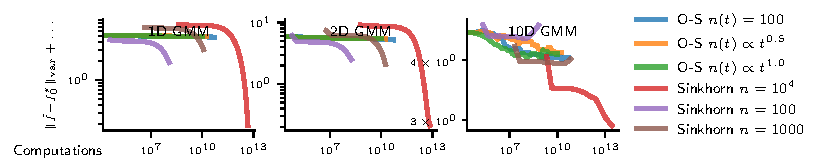
\includegraphics{online_0.0001_True_test}
    \caption{Performance of fully-corrective online Sinkhorn for various $\varepsilon$.}
    \label{fig:convergence_refit}
\end{figure}

\begin{figure}[t]
    
    \caption{Performance of randomized Sinkhorn for various $\varepsilon$.}
    \label{fig:convergence_randomized}
\end{figure}

\begin{figure}[t]
    \caption{Performance of online-Sinkhorn on two Gaussians.}
    \label{fig:gaussian}
\end{figure}

\paragraph{Grids and details for \autoref{sec:online_exp}.} We use $\eta_t, n(t)
= \frac{1}{(1 + 0.1t)^a}, 100 (1 + 0.1t)^{b}$, with $a, b = 0, 2$, $a, b =
\frac{1}{2}, 1$ and $a,b =1, 0$ (constant batch-sizes). We train Sinkhorn on $t
= 5000$ iterations, and O-S to match the number of computations of the large
Sinkhorn reference.

\paragraph{All O-S convergence curves.} To complete \autoref{fig:convergence}, \autoref{fig:convergence_all} report the
performance of online Sinkhorn for $\varepsilon \in [10^{-4}, 10^{-3}, 10^{-2},
10^{-1}]$. The comparison of performance remains similar to the one produced in the main text.

\paragraph{Fully-corrective online Sinkhorn.}\autoref{fig:convergence_refit} reports the performance of
fully-corrected online Sinkhorn (FC-OS). We observe that the fully-corrective scheme is less noisy than the
non-corrected one. It is less efficient than O-S on low-dimensional problems,
but faster on the 10 dimensional problem. For GMM-10D, it outperforms the batch Sinkhorn algorithm
with $N=100, 1000$. Note that we interrupt FC-OS for $n_t > 20,000$, as our implementation of the $C$-transform has a quadratic memory cost in $n_t$---that can be made linear with more care \cite{}.

\paragraph{Randomized Sinkhorn.}\autoref{fig:convergence_randomized} reports
the performance of randomized Sinkhorn.

\paragraph{OT between Gaussians}\autoref{fig:gaussian} reports the performance of online Sinkhorn to transform one Gaussian distribution $\alpha$ to another $\beta$. Potentials are known exactly for this problem, which allows to have a strong golden standard.

\subsection{Illustration of online-Sinkhorn potentials on a 2D GMM}

\begin{figure}[htbp]
    \centering
    
    \caption{Displacement field as defined by the potentials estimated by online-Sinkhorn on a 2D GMM.}
    \label{fig:potentials_2d}
\end{figure}


\subsection{All convergence curves for online Sinkhorn as a warmup process}\label{app:online_exp}


\begin{figure}[t]
    \centering
    $\varepsilon = 0.1$

    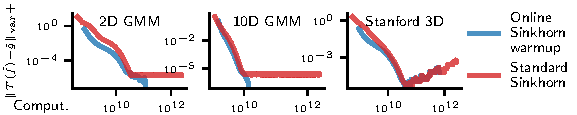
\includegraphics{online+full_0.1_err}
    
    $\varepsilon = 0.01$

    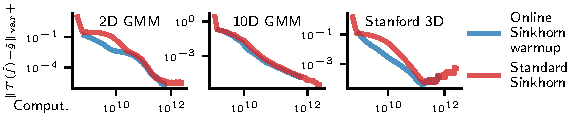
\includegraphics{online+full_0.01_err}

    $\varepsilon = 0.001$

    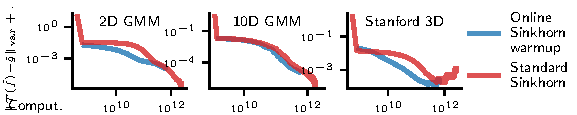
\includegraphics{online+full_0.001_err}

    $\varepsilon = 0.0001$

    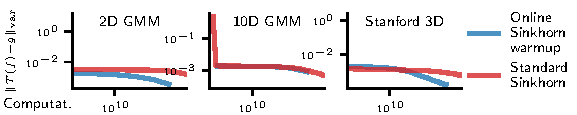
\includegraphics{online+full_0.0001_err}
    \caption{Performance of online-Sinkhorn as warmup for various $\varepsilon$.}
    \label{fig:warmup_full}
\end{figure}

\paragraph{Grids and details for \autoref{sec:online_exp}.} We use $\eta_t, n(t)
= \frac{1}{(1 + 0.1t)^a}, 100 (1 + 0.1t)^{b}$, with $a, b = 0, 2$, $a, b =
\frac{1}{2}, 1$ and $a,b =1, 0$ (constant batch-sizes). We evaluated O-S and
fully-corrective O-S, and found that fully-corrective was less efficient (due to
its higher cost in the early iterations). We evaluated sampling with and without
replacement in the warmyp phase, and found sampling without replacement to be
more efficient.

\paragraph{All warmup convergence curves.} To complete \autoref{fig:warmup}, we report convergence curves for different $\varepsilon$ in \autoref{fig:warmup_full}


\pagebreak

%%%%%%%%%%%%%%%%%%%%%%%%%%%%%%%%%%%%%%%%%%%%%%%%%%%%%%%%
\section{Stochastic mirror descent interpretation}
\label{sec-mirror}

The online Sinkhorn can be understood as a stochastic mirror descent algorithm for a non-convex problem.
%
This equivalence is obtained by applying a change
of variable in \eqref{eq:wass}, defining 
\begin{equation}\label{eq-change-var}
	\mu \triangleq \alpha \exp(f)
	\qandq 
	\nu \triangleq \beta \exp(g). 
\end{equation}
The dual problem~\eqref{eq:dual} 
rewrites as a minimisation problem over positive measures on $\Xx$ and $\Yy$:
\begin{equation}\label{eq:wass_reparam}
    - \!\!\!\!\min_{(\mu,\nu) \in \Mm^+(\Xx)^2} \!\!\!\KL(\alpha | \mu)
    + \KL(\beta | \nu) + \dotp{\mu \otimes \nu}{e^{-C}} - 1,
\end{equation}
where the function $\KL: \Pp(\Xx) \times \Mm^+(\Xx) \triangleq \dotp{\alpha}{ \log \frac{\d \alpha}{\d \mu}}$ is the Kullback-Leibler divergence between
$\alpha$ and $\mu$. 
%
This objective is block convex in $\mu$, $\nu$, but not jointly convex. 
%
As we now detail, this problem can be solved using a stochastic mirror descent~\citep{beck2003mirror}, applied here over the Banach space of Radon measures on $\Xx$, equipped with the total variation norm. 

%%%
\paragraph{Mirror maps and gradient.}

For this, we define the (convex) distance generating function $\Mm^+(\Xx)^2 \to \RR$:
\begin{equation}
    \omega(\mu, \nu) \triangleq \KL(\alpha | \mu) + \KL(\beta | \nu).
\end{equation}
The gradient of this function and of its Fenchel conjugate $\omega^\star:
\Cc(\Xx)^2 \to \RR$ yields two \textit{mirror maps}. For all $(\mu, \nu) \in
\Mm^+(\Xx)^2$, $(\varrho, \varphi) \in \Cc(\Xx)^2, \varrho < 0, \varphi < 0$,
\begin{equation}
    \nabla \omega(\mu, \nu) = (- \frac{\d \alpha}{\d \mu}, - \frac{\d \beta}{\d \nu} )
    \qquad \nabla \omega^\star(\varrho, \varphi)
     = (-\frac{\alpha}{\varrho}, -\frac{\beta}{\varphi}).
\end{equation}
The gradient $\nabla F(\mu, \nu)$ of the objective $F$ appearing
in~\eqref{eq:wass_reparam} is a continuous function
\begin{equation}
    \nabla_\mu F(\mu, \nu) = - \frac{1}{\frac{\d\mu}{\d\alpha}} + \int_{y \in \Xx}
    \frac{\d \nu}{\d \beta}(y) \exp(- C(\cdot, y)) \d \beta(y)
\end{equation}
and similarly for $\nabla_\nu F$.

%%%
\paragraph{Stochastic mirror descent.}

To define stochastic mirror descent iterations, we may replace integration over $\beta$ is by an integration over a sampled measure $\hat \beta$. This in turn defines an \textit{unbiased gradient estimate} $\tilde \nabla F$ of $\nabla F$, which has bounded second order moments.
%
This absence of bias is crucial to prove convergence of SMD with high
probability. Using the mirror maps and the stochastic estimation of the
gradient, one has the following equivalence result, whose proofs stems from
direct computations. 

\begin{proposition}
The stochastic mirror descent iterations
\begin{equation}
    (\mu_t, \nu_t) = \nabla \omega^\star\Big( \nabla \omega(\mu_t, \nu_t) - 
    \eta_t \tilde \nabla F(\mu_t, \nu_t)\Big)
\end{equation}
are equal to the updates~\eqref{eq:updates} under the change of variable~\eqref{eq-change-var}.
\end{proposition}

%%%
\paragraph{Interpretation.} 

It is important to realize that $\mu_t$ and $\nu_t$ do not need to be stored in memory. Instead,
their associated potentials $f_t$ and $g_t$ are parametrized as
\eqref{eq:param}. In particular, $\mu_t$ and $\nu_t$ remain absolutely
continuous with respect to $\alpha$ and $\beta$ respectively, so that the
Kullbach-Leibler divergence terms are always finite. Note that the mirror descent
we consider operates in an infinite-dimensional space, as in \citet{hsieh2018finding}.

Finally, we mention that  when computing exact gradients (in the absence of noise) and when using constant step-size of
$\eta_t=1$, the algorithm matches exactly Sinkhorn iterations with simultaneous updates of the dual variables. This provides a novel interpretation on the Sinkhorn algorithm, that differs from the usual Bregman projection \citep{benamou2015iterative}, and the related understanding of Sinkhorn as a constant step-size mirror descent on the primal objective~\citep{mishchenko2019sinkhorn} and on a semi-dual formulation~\citep{leger2019sinkhorn}. 

Note that one can not directly apply the proofs of convergence of mirror descent to our problem, as the lack of convexity of problem \eqref{eq:wass_reparam} prevents their use.



% \section{Experiments}\label{sec:supp_exp}

% We report the performance of online+full Sinkhorn for $\epsilon \sim 10^{-4}
% \max C$ in \autoref{fig:early_compute_low_eps}. Although the gains are less
% important than with higher $\varepsilon$, they remain significant in this low
% regularization regime.

% \paragraph{Grids in \autoref{sec:exp1}.} We run the online Sinkhorn algorithm
% with step-sizes $\eta_t = \frac{1}{t^a}$, $a \in \{ \frac{1}{2}, 1 \}$
% and $w_t = \frac{1}{{t^b}}$, $b \in \{ \frac{1}{2}, 1 \}$. In all
% experiments, $a = b = \frac{1}{2}$ turned out to perform best.

% \begin{figure}[ht]
%     \centering
%     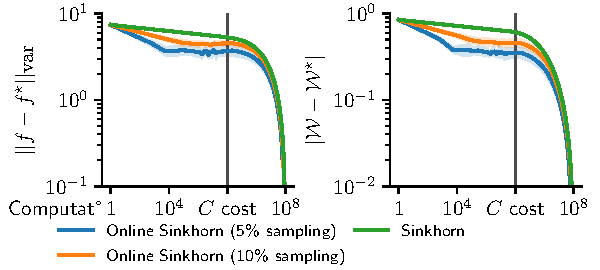
\includegraphics[width=.8\textwidth]{early_compute_low_eps.pdf}
%     \caption{Online Sinkhorn accelerates the first Sinkhorn iterations even for low regularization. $\varepsilon = 10^{-4} \max C$.}
%     \label{fig:early_compute_low_eps}
% \end{figure}
